\documentclass[t aspectratio=169]{beamer}
\usetheme{Rochester}
\usecolortheme{seahorse}
\usepackage{attachfile}
\usepackage{fontawesome5}
\usepackage{cmap}
\usepackage{mathtext}
\usepackage[T2A]{fontenc}
\usepackage[utf8]{inputenc}
\usepackage[english,russian]{babel}
\title{Изучение методов фрактального сжатия для различных типов информации}
% \author[author1]{Милов Данила Константинович\\[10mm]{\small Руководитель: Дудаков Сергей Михайлович}}
\date{\today}
\begin{document}
  \begin{frame}
    \maketitle
  \end{frame}

  \section*{Оглавление}
  \begin{frame}\frametitle{\insertsection}
    \large
    \tableofcontents
    \normalfont
  \end{frame}

  \section{Актуальность работы}
  \begin{frame}\frametitle{\insertsection}
    \begin{columns}
      \column{0.5\textwidth}
      \begin{figure}
        \begin{center}
          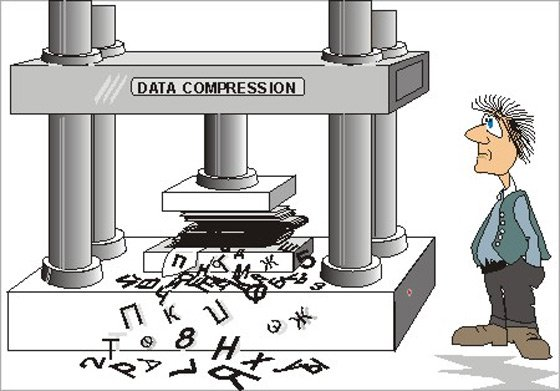
\includegraphics[width=1\textwidth]{./images/compression-illustration.jpg}
        \end{center}
      \end{figure}
      \column{0.5\textwidth}
      \large Плюсы сжатия информации:
      \begin{itemize}
        \item Уменьшение занимаемого места на диске.
        \item Ускорение передачи данных за счёт меньшего объёма файлов.
        \item Более низкие затраты на хранение и пропускную способность.
      \end{itemize}
    \normalsize
    \end{columns}
  \end{frame}

  \section{Цели и задачи}
  \begin{frame}\frametitle{\insertsection}
    \large
    \begin{block}{Цель работы}
      Изучить и реализовать алгоритмы фрактального сжатия для различных типов информации
    \end{block}

    \vspace{1em}
    \textbf{Задачи}
    \begin{enumerate}
      \item Изучение алгоритмов фрактального сжатия изображений и звука.
      \item Реализовать изученные алгоритмы.
      \item Сравнить качество сжимающих алгоритмов.
    \end{enumerate}
    \normalfont
  \end{frame}

  \section{Иллюстрация алгоритма}
  \begin{frame}\frametitle{\insertsection}

  \end{frame}

  \section{CLI-интерфейс сжатия изображений}
  \begin{frame}\frametitle{\insertsection}
   \begin{figure}
    \begin{center}
      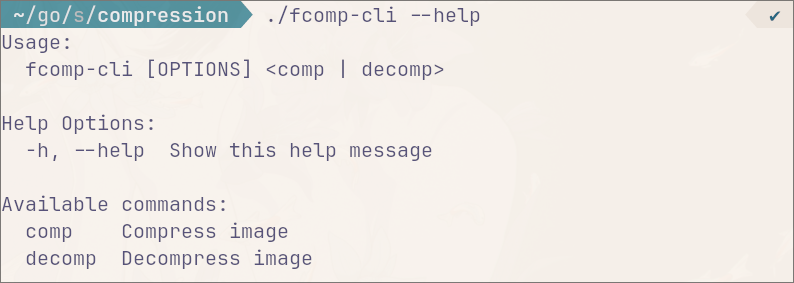
\includegraphics[width=\textwidth]{./images/cli-main.png}
    \end{center}
   \end{figure}
  \end{frame}

  \begin{frame}\frametitle{\insertsection. Команда comp}
   \begin{figure}
    \begin{center}
      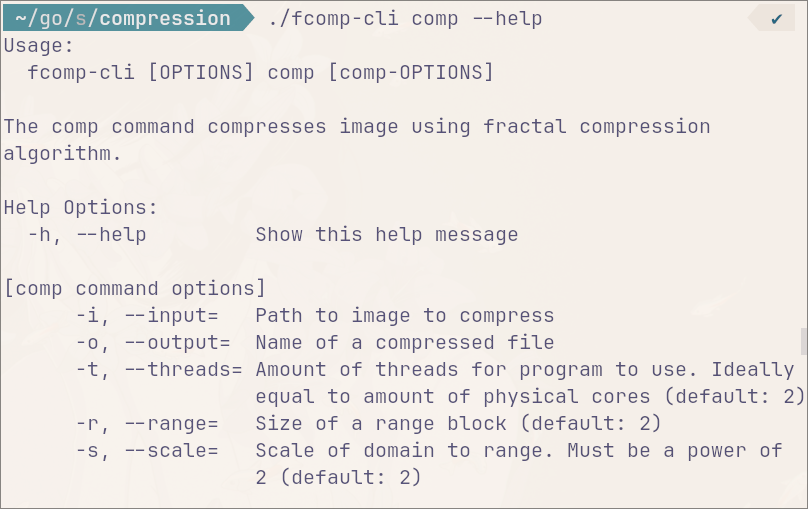
\includegraphics[width=\textwidth]{./images/cli-comp.png}
    \end{center}
   \end{figure}
  \end{frame}

  \begin{frame}\frametitle{\insertsection. Команда decomp}
   \begin{figure}
    \begin{center}
      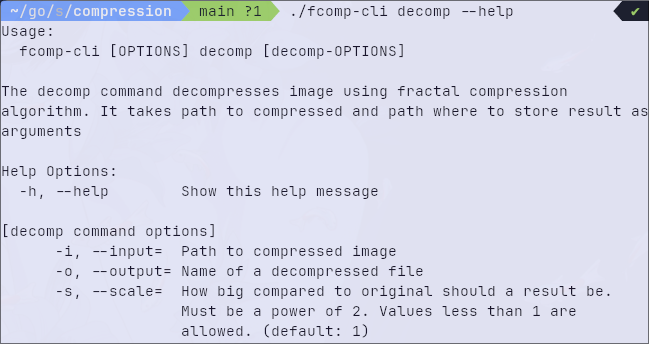
\includegraphics[width=\textwidth]{./images/cli-decomp.png}
    \end{center}
   \end{figure}
  \end{frame}

  \section{Пример работы программы}
  \begin{frame}\frametitle{\insertsection}
    Work In Progress
  \end{frame}

  \section*{Спасибо за внимание!}
  \begin{frame}
    \begin{center}
      \huge Спасибо за внимание!\normalfont
    \end{center}
  \end{frame}

\end{document}
